\documentclass[conference]{IEEEtran}
\IEEEoverridecommandlockouts
% The preceding line is only needed to identify funding in the first footnote. If that is unneeded, please comment it out.
\usepackage{cite}
\usepackage{amsmath,amssymb,amsfonts}
\usepackage{algorithmic}
\usepackage{graphicx}
\usepackage{textcomp}
\usepackage{xcolor}
\def\BibTeX{{\rm B\kern-.05em{\sc i\kern-.025em b}\kern-.08em
    T\kern-.1667em\lower.7ex\hbox{E}\kern-.125emX}}
\graphicspath{{Figures/}}

\begin{document}

\title{Secure Industrial Control System with Intrusion Detection\\
% {\footnotesize \textsuperscript{*}Note: Sub-titles are not captured in Xplore and
% should not be used}
}

\author{\IEEEauthorblockN{1\textsuperscript{st} Given Name Surname}
\IEEEauthorblockA{\textit{dept. name of organization (of Aff.)} \\
\textit{name of organization (of Aff.)}\\
City, Country \\
email address}
\and
\IEEEauthorblockN{Denis Ulybyshev}
\IEEEauthorblockA{\textit{Computer Science Department, CEROC} \\
\textit{Tennessee Technological University}\\
Cookeville, TN, United States of America \\
dulybyshev@tntech.edu}
\and
\IEEEauthorblockN{3\textsuperscript{rd} Given Name Surname}
\IEEEauthorblockA{\textit{dept. name of organization (of Aff.)} \\
\textit{name of organization (of Aff.)}\\
City, Country \\
email address}
\and
\IEEEauthorblockN{4\textsuperscript{th} Given Name Surname}
\IEEEauthorblockA{\textit{dept. name of organization (of Aff.)} \\
\textit{name of organization (of Aff.)}\\
City, Country \\
email address}
\and
\IEEEauthorblockN{5\textsuperscript{th} Given Name Surname}
\IEEEauthorblockA{\textit{dept. name of organization (of Aff.)} \\
\textit{name of organization (of Aff.)}\\
City, Country \\
email address}
\and
\IEEEauthorblockN{6\textsuperscript{th} Given Name Surname}
\IEEEauthorblockA{\textit{dept. name of organization (of Aff.)} \\
\textit{name of organization (of Aff.)}\\
City, Country \\
email address}
}

\maketitle

\begin{abstract}

\end{abstract}

\begin{IEEEkeywords}

\end{IEEEkeywords}

\section{Introduction}
Industrial control system (ICS) is the technology used to automate the manufacturing process. It is responsible for controlling and managing large number of field devices. The manufacturing industry has seen an astronomical rise in the adoption of ICS in recent years. The fierce competition among the companies has been the main catalyst for this revolution in the manufacturing industry. According to the study report published by  Market Research Future (MRFR), the industrial control system market will be growing even more in the future \cite{c1}. A lot of these industrial control system are deployed in critical infrastructures such as the smart grid, health care system, water purification, nuclear plants. As a result, any kind of security breach and attack can have significant impact on human lives as well as be very costly. Securing these system has become a priority as a result of the increasing number of attacks in these domain. 
\section{Related Work}


\section{Security in ICS}
\begin{figure}[htbp]
\centering
\centerline{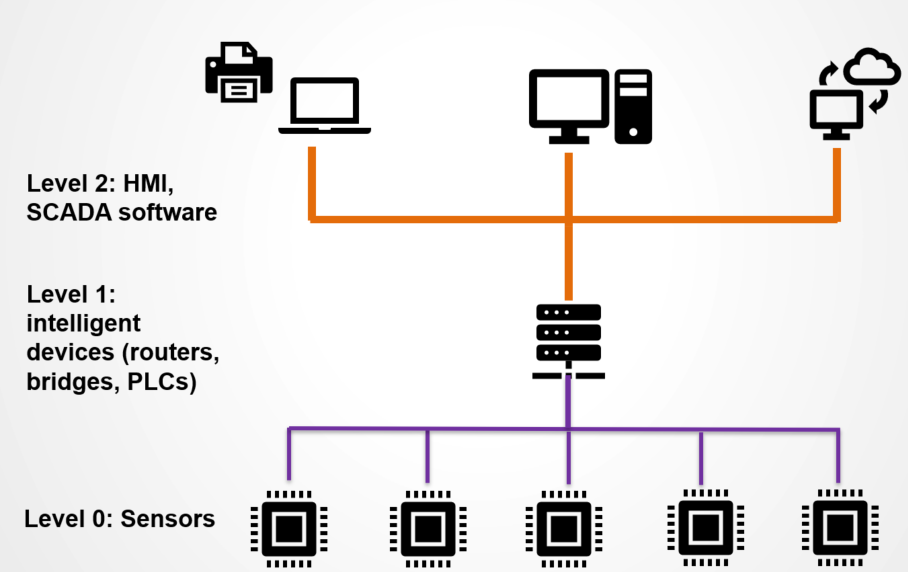
\includegraphics [width=9cm] {Architecture1.png}}
\caption{Industrial Control System Architecture}
\label{fig}
\end{figure}


\subsection{Software Solutions}\label{AA}

\subsection{Observed Gap}

\section{Proposed Architecture}

\section{Work in Progress and Future Direction}

\section{Conclusion}




\begin{thebibliography}{00}
\bibitem{c1}Industrial Control Systems (ICS) Market 2018 Global Analysis, Industry Size, Share Leaders, Current Status by Major Key vendors and Trends by Forecast to 2023. https://www.marketwatch.com/press-release/industrial-control-systems-ics-market-2018-global-analysis-industry-size-share-leaders-current-status-by-major-key-vendors-and-trends-by-forecast-to-2023-2018-11-29
\end{thebibliography}
\vspace{12pt}
\end{document}
